% =====================================================================
% Guía del estudiante -- Geometría 3° -- Trimestre I
% Hilo conductor: Rinrín Renacuajo sale de paseo (versión propia, sin el final del poema)
% Temas (propuesta del trimestre I en curriculo/plan-anual.md, clases 003-011):
%   lineas, figuras, cuerpos, formas
% Plan y ejercicios: guia-periodo-I-del-punto-al-cuerpo.plan.md
% =====================================================================
% Plan del trimestre aprobado por la docente el 2026-09-18. Esta guía es todavía el borrador de
% la generación rápida del 2026-09-14: falta rehacerla con el proceso de tres etapas.
\documentclass[11pt]{article}
\makeatletter\def\input@path{{../../../../plantillas/estilo/}}\makeatother
\usepackage{mmcantillo}

% ======================== DATOS DE LA GUÍA ============================
\tipodocumento{Guía del estudiante}
\asignatura{Geometría}
\titulo{Del punto al cuerpo}
\grado{3°}
\periodo{I}
\hiloconductor{Rinrín Renacuajo sale de paseo}
% ======================================================================
% DBA: matematicas grado 3 · DBA 6 — Describe y representa formas bidimensionales y
% tridimensionales de acuerdo con las propiedades geométricas. (dba/matematicas/grados/grado03.tex)

\tikzset{etq/.style={font=\small\bfseries, text height=1.6ex, text depth=0.3ex}}

\begin{document}

\encabezado

% ---------------------------------------------------------------------
% 1. Frase introductoria
% ---------------------------------------------------------------------
% verificado: https://babel.banrepcultural.org/digital/api/collection/p17054coll10/id/2720/download — Cuentos pintados para niños (1867), versos iniciales de «El renacuajo paseador»; texto contrastado en https://es.wikisource.org/wiki/El_renacuajo_paseador
\frase{El hijo de Rana, Rinrín Renacuajo, salió esta mañana muy tieso y
muy majo, con pantalón corto, corbata a la moda, sombrero encintado y
chupa de boda.}
{Rafael Pombo, \emph{El renacuajo paseador} (1867)}

% ---------------------------------------------------------------------
% 2. Introducción
% ---------------------------------------------------------------------
\seccion{Introducción}

¿Te acuerdas del punto de luz del láser en la pared? Con puntos se hacen
líneas. Con líneas se hacen figuras. Y con figuras se arman cuerpos, como
una caja o un dado. En este trimestre vamos a hacer ese viaje:
\textbf{del punto al cuerpo}.

Te acompañará Rinrín Renacuajo, el personaje del poeta colombiano Rafael
Pombo~\cite{pombo}. En nuestra versión del cuento, Rinrín sale de su charco
a pasear. Deja caminos en la arena, visita la casa de Doña Ratona y pasa por
la tienda del barrio. ¡En todas partes encuentra formas!

\textbf{Al terminar este trimestre podrás:}
\begin{itemize}
  \item reconocer líneas rectas y curvas, abiertas y cerradas;
  \item nombrar figuras planas y contar sus lados y vértices;
  \item reconocer cuerpos geométricos y contar sus caras, aristas y vértices;
  \item clasificar formas y decir qué regla usaste.
\end{itemize}

Este es el aprendizaje que el Ministerio de Educación espera para tu
grado~\cite{mendba}:

\begin{dba}[Grado 3 · DBA 6]
Describe y representa formas bidimensionales y tridimensionales de acuerdo
con las propiedades geométricas.
\end{dba}

% ---------------------------------------------------------------------
% 3. Marco teórico (en 3°: anécdotas, sin citas textuales)
% ---------------------------------------------------------------------
\seccion{Marco teórico: ¿Sabías que\ldots?}

\subsubsection*{El poeta que estudió matemáticas}
Rafael Pombo nació en Bogotá en 1833. Antes de escribir cuentos para niños,
estudió \textbf{matemáticas e ingeniería}. Sus \emph{Cuentos pintados para
niños}, donde vive Rinrín, se publicaron en 1867~\cite{banrep}. ¡Un poeta
que sabía geometría!

\subsubsection*{Un libro de formas muy, muy antiguo}
Hace más de 2\,000 años, un maestro griego llamado \textbf{Euclides}
escribió un libro sobre las formas: los \emph{Elementos}. Empieza así: un
\textbf{punto} es algo que no tiene partes, y una \textbf{línea} es un largo
sin ancho~\cite{euclides}. Con puntos y líneas se arman todas las figuras.

\subsubsection*{Las abejas también saben geometría}
Las abejas hacen sus panales con celdas de \textbf{seis lados}. En el año
2001, el matemático Thomas Hales demostró que los hexágonos dividen un piso
en partes iguales usando el borde más corto posible. Por eso se piensa que
así las abejas ahorran cera~\cite{hales}.

% ---------------------------------------------------------------------
% 4. Temas
% ---------------------------------------------------------------------
\tema{Líneas}\label{tema:lineas}

\begin{hilo}
Rinrín sale muy elegante de su charco. Camina por la arena y deja caminos:
unos derechitos, otros con curvas. Algunos caminos vuelven al charco y otros
no. «¿Cómo se llamarán?», piensa Rinrín.
\end{hilo}

Si mueves el punto de luz del láser por la pared, dibujas una
\textbf{línea}. Hay dos clases de líneas:

\begin{center}
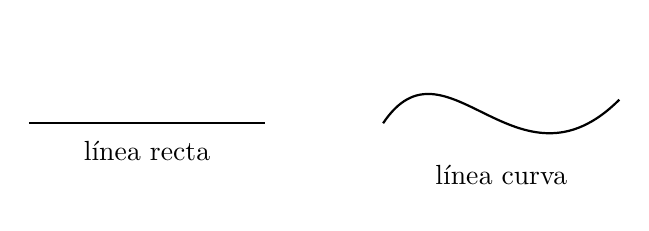
\begin{tikzpicture}[thick]
  \draw (0,0) -- (3,0);            \node[below] at (1.5,-0.1) {línea recta};
  \draw (4.5,0) .. controls (5.3,1.2) and (6.2,-1) .. (7.5,0.3);
                                   \node[below] at (6,-0.4) {línea curva};
\end{tikzpicture}
\end{center}

Las líneas rectas pueden estar en distintas posiciones:
\textbf{horizontal}, como el piso; \textbf{vertical}, como un poste; o
\textbf{inclinada}, como una escoba recostada en la pared.

\begin{center}
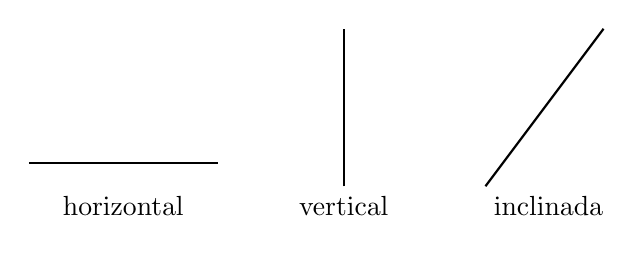
\begin{tikzpicture}[thick, every node/.append style={text height=1.6ex, text depth=0.3ex}]
  \draw (0,0) -- (2.4,0);    \node[below] at (1.2,-0.3) {horizontal};
  \draw (4,-0.3) -- (4,1.7); \node[below] at (4,-0.3) {vertical};
  \draw (5.8,-0.3) -- (7.3,1.7); \node[below] at (6.6,-0.3) {inclinada};
\end{tikzpicture}
\end{center}

Una línea es \textbf{cerrada} si termina en el mismo punto donde empezó, sin
levantar el lápiz. Si no, es \textbf{abierta}.

\begin{center}
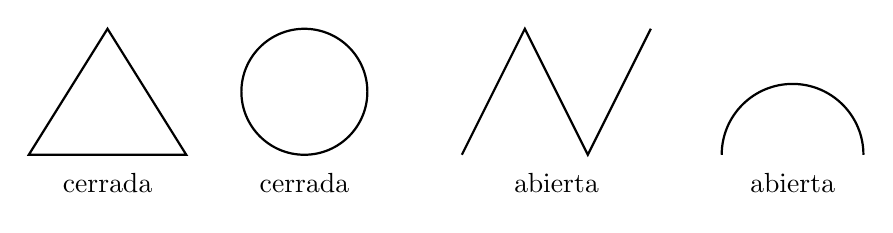
\begin{tikzpicture}[thick, every node/.append style={text height=1.6ex, text depth=0.3ex}]
  \draw (0,0) -- (2,0) -- (1,1.6) -- cycle;   \node[below] at (1,-0.1) {cerrada};
  \draw (3.5,0.8) circle (0.8);               \node[below] at (3.5,-0.1) {cerrada};
  \draw (5.5,0) -- (6.3,1.6) -- (7.1,0) -- (7.9,1.6); \node[below] at (6.7,-0.1) {abierta};
  \draw (10.6,0) arc (0:180:0.9);             \node[below] at (9.7,-0.1) {abierta};
\end{tikzpicture}
\end{center}

Una línea cerrada separa lo que está \textbf{dentro}, lo que está
\textbf{fuera} y lo que está justo \textbf{en el borde}.

\begin{ejemplo}[El charco de Rinrín]
El borde del charco es una línea cerrada. Rinrín, nadando, está
\emph{dentro}. Una piedra en la orilla está \emph{en el borde}. El árbol del
parque está \emph{fuera}.
\end{ejemplo}

\begin{aplicacion}[La cancha del colegio]
Las líneas blancas de la cancha forman una línea cerrada. Así, el árbitro
sabe si el balón está dentro o fuera. ¡Si toca la línea, está en el borde,
y en muchos deportes todavía cuenta como dentro!
\end{aplicacion}

\begin{preguntas}
% Ejercicio: lineas-3-002
\pregunta Escribe al lado de cada número si la línea es horizontal,
vertical o inclinada.
\begin{center}
\begin{tikzpicture}[thick, scale=0.95]
  \draw (0,0) -- (3,0);   \node[etq, above] at (1.5,0.05) {1};
  \draw (4,0) -- (4,2);   \node[etq, left] at (4,1) {2};
  \draw (5,0) -- (7,2);   \node[etq, right] at (6.1,0.9) {3};
  \draw (8,2) -- (11,2);  \node[etq, below] at (9.5,1.95) {4};
\end{tikzpicture}
\end{center}
1: \rule{2.4cm}{0.4pt} \quad 2: \rule{2.4cm}{0.4pt} \quad
3: \rule{2.4cm}{0.4pt} \quad 4: \rule{2.4cm}{0.4pt}

\Needspace{12\baselineskip}
% Ejercicio: lineas-3-004
\pregunta El borde del charco de Rinrín es una línea cerrada. ¿Quién está
dentro del charco, quién está fuera y quién está justo en el borde?
\begin{center}
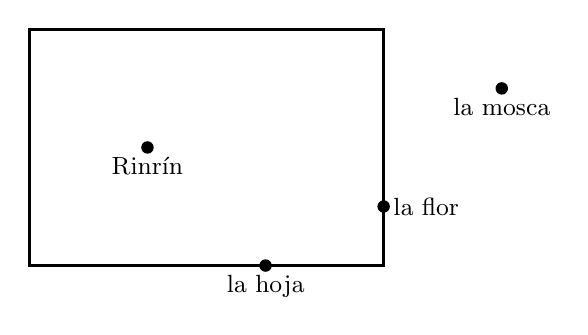
\begin{tikzpicture}[scale=0.75, every node/.append style={font=\small}]
  \draw[very thick] (0,0) rectangle (6,4);
  \fill (2,2) circle (3pt) node[below] {Rinrín};
  \fill (8,3) circle (3pt) node[below] {la mosca};
  \fill (6,1) circle (3pt) node[right] {la flor};
  \fill (4,0) circle (3pt) node[below] {la hoja};
\end{tikzpicture}
\end{center}
Dentro: \rule{2.8cm}{0.4pt} \quad Fuera: \rule{2.8cm}{0.4pt} \quad
En el borde: \rule{2.8cm}{0.4pt}
\end{preguntas}

\begin{resumen}
\begin{itemize}
  \item Las líneas pueden ser \textbf{rectas} o \textbf{curvas}.
  \item Una recta puede estar \textbf{horizontal}, \textbf{vertical} o \textbf{inclinada}.
  \item Una línea \textbf{cerrada} termina donde empezó; separa lo de dentro,
        lo de fuera y el borde. Si no termina donde empezó, es \textbf{abierta}.
\end{itemize}
\end{resumen}

% ---------------------------------------------------------------------
\tema{Figuras planas}\label{tema:figuras}

\begin{hilo}
En el camino, Rinrín se encuentra con su vecino, el Ratón. «¡Amigo, venga
usted conmigo!», le dice. Juntos van a visitar a Doña Ratona. Su casa está
hecha de formas: un techo, una pared, una puerta y ventanas.
\end{hilo}

Cuando una línea cerrada encierra un pedazo de la hoja, tenemos una
\textbf{figura plana}. Estas son cuatro muy importantes:

\begin{center}
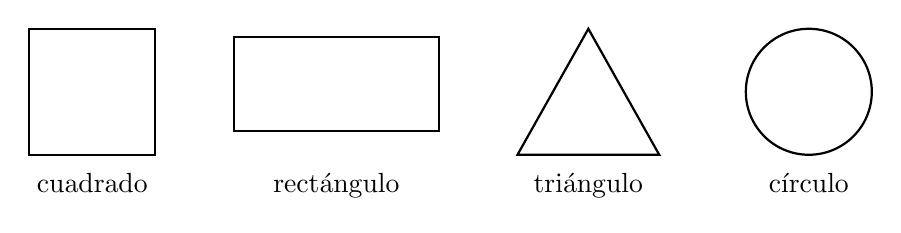
\begin{tikzpicture}[thick, every node/.append style={text height=1.6ex, text depth=0.3ex}]
  \draw (0,0) rectangle (1.6,1.6);          \node[below] at (0.8,-0.1) {cuadrado};
  \draw (2.6,0.3) rectangle (5.2,1.5);      \node[below] at (3.9,-0.1) {rectángulo};
  \draw (6.2,0) -- (8.0,0) -- (7.1,1.6) -- cycle; \node[below] at (7.1,-0.1) {triángulo};
  \draw (9.9,0.8) circle (0.8);             \node[below] at (9.9,-0.1) {círculo};
\end{tikzpicture}
\end{center}

Cada línea recta del borde es un \textbf{lado}. El punto donde se juntan dos
lados es un \textbf{vértice} (una esquina). El círculo no tiene lados rectos
ni vértices.

\begin{center}
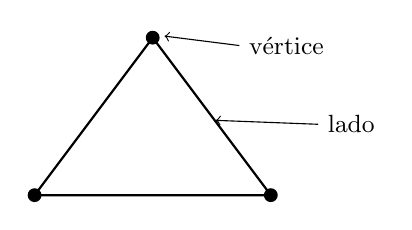
\begin{tikzpicture}[thick]
  \draw (0,0) -- (3,0) -- (1.5,2) -- cycle;
  \foreach \p in {(0,0),(3,0),(1.5,2)} \fill \p circle (2.5pt);
  \draw[->, thin] (2.6,1.9) node[right, font=\small] {vértice} -- (1.65,2.02);
  \draw[->, thin] (3.6,0.9) node[right, font=\small] {lado} -- (2.3,0.95);
\end{tikzpicture}
\end{center}

\begin{ejemplo}[Contar y comparar]
El triángulo tiene \textbf{3 lados} y \textbf{3 vértices}. El cuadrado y el
rectángulo tienen \textbf{4 lados} y \textbf{4 vértices}. ¿En qué se
diferencian? Los 4 lados del cuadrado miden lo mismo; el rectángulo tiene
dos lados largos y dos cortos.
\end{ejemplo}

Para \textbf{clasificar} figuras hacemos grupos con una regla, por ejemplo
«las que tienen 3 lados» y «las que tienen 4 lados». Siempre hay que decir
qué regla usamos.

\begin{aplicacion}[Señales de tránsito]
Las señales tienen formas distintas para que los conductores las reconozcan
desde lejos. La señal de \textbf{PARE} tiene 8 lados. La de \textbf{CEDA EL
PASO} es un triángulo. ¡Hasta sin leerlas sabemos qué dicen!
\end{aplicacion}

\begin{preguntas}
\Needspace{14\baselineskip}
% Ejercicio: figuras-planas-3-003
\pregunta Separa las seis figuras en grupos según su número de lados.
Escribe qué regla usaste.
\begin{center}
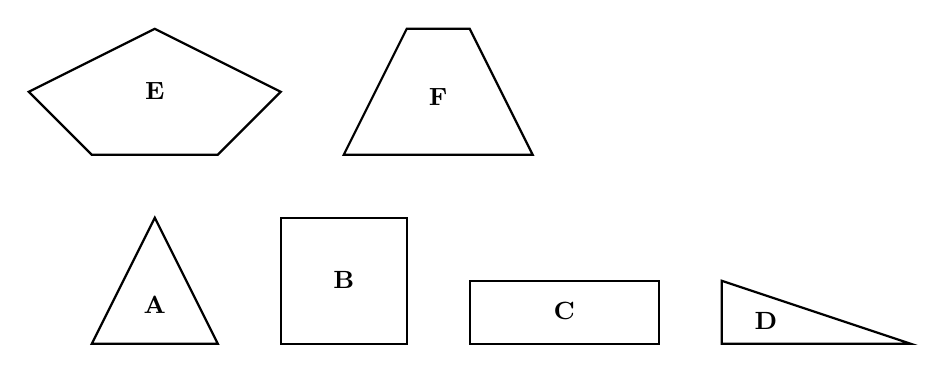
\begin{tikzpicture}[thick, scale=0.8]
  \draw (0,0) -- (2,0) -- (1,2) -- cycle;                   \node[etq] at (1,0.6) {A};
  \draw (3,0) rectangle (5,2);                              \node[etq] at (4,1) {B};
  \draw (6,0) rectangle (9,1);                              \node[etq] at (7.5,0.5) {C};
  \draw (10,0) -- (13,0) -- (10,1) -- cycle;                \node[etq] at (10.7,0.35) {D};
  \draw (0,3) -- (2,3) -- (3,4) -- (1,5) -- (-1,4) -- cycle; \node[etq] at (1,4) {E};
  \draw (4,3) -- (7,3) -- (6,5) -- (5,5) -- cycle;          \node[etq] at (5.5,3.9) {F};
\end{tikzpicture}
\end{center}
\renglones{3}

\Needspace{9\baselineskip}
% Ejercicio: figuras-planas-3-004
\pregunta El Ratón mira esta figura y dice: «No es un cuadrado, porque está
de punta». ¿Tiene razón? Explica.
\begin{center}
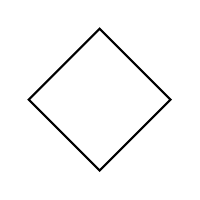
\begin{tikzpicture}[thick, scale=0.45]
  \draw (2,0) -- (4,2) -- (2,4) -- (0,2) -- cycle;
\end{tikzpicture}
\end{center}
\renglones{2}
\end{preguntas}

\begin{resumen}
\begin{itemize}
  \item Una figura plana está encerrada por una línea cerrada: cuadrado,
        rectángulo, triángulo, círculo\ldots
  \item Los \textbf{lados} son las líneas rectas del borde; los
        \textbf{vértices} son las esquinas donde se juntan dos lados.
  \item Girar una figura no cambia su nombre.
  \item Para clasificar, hacemos grupos con una regla y decimos cuál es.
\end{itemize}
\end{resumen}

% ---------------------------------------------------------------------
\tema{Cuerpos geométricos}\label{tema:cuerpos}

\begin{hilo}
Después de la visita, Rinrín pasa por la tienda del barrio. Ve cajas de
cereal, latas de atún, pelotas y conos de helado. «Estas formas no son
planas», piensa. «¡Se pueden agarrar con las manos!»
\end{hilo}

Los \textbf{cuerpos geométricos} no caben en una hoja: tienen largo, ancho
y alto. Estos son algunos:

\begin{center}
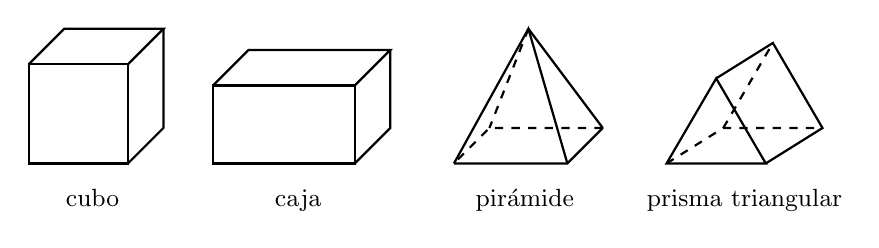
\begin{tikzpicture}[thick, scale=0.9, every node/.append style={text height=1.6ex, text depth=0.3ex, font=\small}]
  % cubo
  \draw (0,0) rectangle (1.4,1.4);
  \draw (0,1.4) -- (0.5,1.9) -- (1.9,1.9) -- (1.4,1.4);
  \draw (1.9,1.9) -- (1.9,0.5) -- (1.4,0);
  \node[below] at (0.9,-0.2) {cubo};
  % caja
  \begin{scope}[xshift=2.6cm]
    \draw (0,0) rectangle (2,1.1);
    \draw (0,1.1) -- (0.5,1.6) -- (2.5,1.6) -- (2,1.1);
    \draw (2.5,1.6) -- (2.5,0.5) -- (2,0);
    \node[below] at (1.2,-0.2) {caja};
  \end{scope}
  % pirámide
  \begin{scope}[xshift=6cm]
    \draw (0,0) -- (1.6,0) -- (2.1,0.5);
    \draw[dashed] (2.1,0.5) -- (0.5,0.5) -- (0,0);
    \draw (0,0) -- (1.05,1.9) -- (1.6,0);
    \draw (1.05,1.9) -- (2.1,0.5);
    \draw[dashed] (1.05,1.9) -- (0.5,0.5);
    \node[below] at (1,-0.2) {pirámide};
  \end{scope}
  % prisma triangular
  \begin{scope}[xshift=9cm]
    \draw (0,0) -- (1.4,0) -- (0.7,1.2) -- cycle;
    \draw (1.4,0) -- (2.2,0.5) -- (1.5,1.7) -- (0.7,1.2);
    \draw[dashed] (0,0) -- (0.8,0.5) -- (2.2,0.5);
    \draw[dashed] (0.8,0.5) -- (1.5,1.7);
    \node[below] at (1.1,-0.2) {prisma triangular};
  \end{scope}
\end{tikzpicture}

\medskip
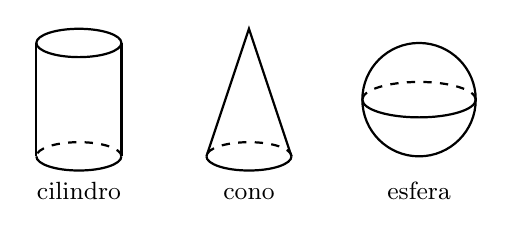
\begin{tikzpicture}[thick, scale=0.9, every node/.append style={text height=1.6ex, text depth=0.3ex, font=\small}]
  % cilindro
  \draw (0,1.6) ellipse (0.6 and 0.2);
  \draw (-0.6,1.6) -- (-0.6,0);  \draw (0.6,1.6) -- (0.6,0);
  \draw (-0.6,0) arc (180:360:0.6 and 0.2);
  \draw[dashed] (0.6,0) arc (0:180:0.6 and 0.2);
  \node[below] at (0,-0.2) {cilindro};
  % cono
  \begin{scope}[xshift=2.4cm]
    \draw (-0.6,0) -- (0,1.8) -- (0.6,0);
    \draw (-0.6,0) arc (180:360:0.6 and 0.2);
    \draw[dashed] (0.6,0) arc (0:180:0.6 and 0.2);
    \node[below] at (0,-0.2) {cono};
  \end{scope}
  % esfera
  \begin{scope}[xshift=4.8cm]
    \draw (0,0.8) circle (0.8);
    \draw (-0.8,0.8) arc (180:360:0.8 and 0.25);
    \draw[dashed] (0.8,0.8) arc (0:180:0.8 and 0.25);
    \node[below] at (0,-0.2) {esfera};
  \end{scope}
\end{tikzpicture}
\end{center}

Las partes de un cuerpo tienen nombre. Cada superficie plana es una
\textbf{cara}; ¡y cada cara es una figura plana! El borde donde se juntan
dos caras es una \textbf{arista}. La punta donde se juntan varias aristas es
un \textbf{vértice}. (Las líneas punteadas del dibujo son las aristas que
quedan atrás y no se ven.)

\begin{center}
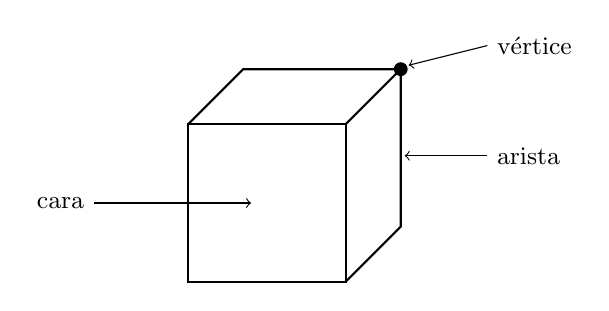
\begin{tikzpicture}[thick]
  \draw (0,0) rectangle (2,2);
  \draw (0,2) -- (0.7,2.7) -- (2.7,2.7) -- (2,2);
  \draw (2.7,2.7) -- (2.7,0.7) -- (2,0);
  \fill (2.7,2.7) circle (2.5pt);
  \draw[->, thin] (3.8,3) node[right, font=\small] {vértice} -- (2.8,2.75);
  \draw[->, thin] (3.8,1.6) node[right, font=\small] {arista} -- (2.75,1.6);
  \draw[->, thin] (-1.2,1) node[left, font=\small] {cara} -- (0.8,1);
\end{tikzpicture}
\end{center}

\begin{ejemplo}[Las caras son figuras planas]
Las 6 caras del cubo son cuadrados. La pirámide tiene una cara cuadrada (la
base) y 4 caras triangulares. El prisma triangular tiene 2 caras
triangulares y 3 rectangulares.
\end{ejemplo}

\begin{ejemplo}[¿Rueda o no rueda?]
El cubo y la caja tienen solo caras planas: \textbf{no ruedan}. La esfera es
toda curva: \textbf{rueda hacia cualquier lado}. El cilindro y el cono tienen
una parte curva: ruedan si los acuestas.
\end{ejemplo}

\begin{aplicacion}[En la tienda]
Las cajas se pueden poner una encima de otra sin que se caigan, porque sus
caras son planas. Por eso los cereales y los zapatos vienen en cajas. Las
latas son cilindros: se paran sobre una cara plana, pero si las acuestas,
¡ruedan!
\end{aplicacion}

\begin{preguntas}
\Needspace{11\baselineskip}
% Ejercicio: cuerpos-geometricos-3-001
\pregunta Completa la tabla. Si puedes, cuenta con un cuerpo de verdad en la
mano.
\begin{center}
{\renewcommand{\arraystretch}{1.8}
\begin{tabular}{|l|c|c|c|}
  \hline
  \textbf{Cuerpo} & \textbf{Caras} & \textbf{Aristas} & \textbf{Vértices}\\\hline
  Cubo                    & \hspace{2cm} & \hspace{2cm} & \hspace{2cm}\\\hline
  Caja                    & & & \\\hline
  Pirámide (base cuadrada) & & & \\\hline
  Prisma triangular        & & & \\\hline
\end{tabular}}
\end{center}

% Ejercicio: cuerpos-geometricos-3-003
\pregunta El Ratón dice: «El dado tiene 6 caras, así que también tiene 6
vértices». ¿Tiene razón? Cuenta en un dado de verdad.
\renglones{2}
\end{preguntas}

\begin{resumen}
\begin{itemize}
  \item Los cuerpos geométricos tienen largo, ancho y alto: cubo, caja,
        pirámide, prisma, cilindro, cono y esfera.
  \item Sus partes son las \textbf{caras} (figuras planas), las
        \textbf{aristas} (bordes) y los \textbf{vértices} (puntas).
  \item Los cuerpos con solo caras planas no ruedan; los que tienen partes
        curvas pueden rodar.
\end{itemize}
\end{resumen}

% ---------------------------------------------------------------------
\tema{Formas a mi alrededor}\label{tema:formas}

\begin{hilo}
Rinrín vuelve a casa y le quiere contar a Mamá Rana todo lo que vio. Pero no
tiene papel para dibujar. ¿Cómo explicarle las formas solo con palabras?
\end{hilo}

Todo lo que nos rodea tiene forma. La tapa de un tarro es un
\textbf{círculo}, y el tarro es un \textbf{cilindro}. La cara de un dado es
un \textbf{cuadrado}, y el dado es un \textbf{cubo}.

Para describir un cuerpo sin dibujarlo, hay que decir:
\begin{itemize}
  \item cuántas caras tiene;
  \item qué figura plana es cada cara;
  \item de qué tamaño son las caras.
\end{itemize}

\begin{ejemplo}[Un buen mensaje]
«Es un cuerpo con 6 caras. Todas son cuadrados iguales, de 3 centímetros de
lado.» Con ese mensaje cualquiera sabe que es un \textbf{cubo} y puede
construirlo.
\end{ejemplo}

\begin{aplicacion}[Instrucciones de armado]
Las cajas de regalo y muchos juguetes traen instrucciones para armarlos.
Unas buenas instrucciones dicen qué piezas hay, qué forma tienen y cómo se
unen. ¡Si faltan datos, el juguete queda mal armado!
\end{aplicacion}

\begin{preguntas}
% Ejercicio: formas-3-001
\pregunta Adivina, adivinador: ¿qué cuerpo soy? Elige entre el cubo, la
caja, la pirámide y el prisma triangular.
\begin{enumerate}[label=\alph*)]
  \item «Tengo 6 caras y todas son cuadrados iguales.» \hfill \rule{3.5cm}{0.4pt}
  \item «Tengo 5 caras: 2 son triángulos y 3 son rectángulos.» \hfill \rule{3.5cm}{0.4pt}
  \item «Tengo 5 caras y 5 vértices; una cara es un cuadrado y las otras son
        triángulos.»\\ \hspace*{\fill}\rule{3.5cm}{0.4pt}
\end{enumerate}

% Ejercicio: formas-3-003 — manual-pendiente (ejemplo del DBA 6 de 3°): entra cuando la
% docente apruebe la respuesta modelo (python3 tools/ejercicios.py aprobar formas-3-003).
% \pregunta David y María faltaron a clase y no vieron los cuerpos que tenía la profesora: una
% caja, un prisma triangular y un cilindro. Escríbeles un mensaje, sin dibujos, para que puedan
% construirlos en cartulina iguales a los de la profesora. \renglones{5}
\end{preguntas}

\begin{resumen}
\begin{itemize}
  \item Los objetos de la casa y del colegio tienen forma de figuras planas
        o de cuerpos geométricos.
  \item Las caras de un cuerpo son figuras planas.
  \item Para describir un cuerpo sin dibujarlo: número de caras, forma de
        cada cara y su tamaño.
\end{itemize}
\end{resumen}

% ---------------------------------------------------------------------
% 5. Cierre del hilo conductor
% ---------------------------------------------------------------------
\seccion{Cierre: Rinrín vuelve a su charco}

En nuestra versión del cuento, Rinrín regresa a su charco antes de que
oscurezca. Mamá Rana lo espera contenta. Esa noche, Rinrín le cuenta todo:
los caminos rectos y curvos, la casa de Doña Ratona llena de figuras y las
cajas y latas de la tienda. ¡Fue un paseo del punto al cuerpo!

En el próximo trimestre vamos a \textbf{medir}: cuánto mide el borde de una
figura y cuántos cuadritos la cubren.

% ---------------------------------------------------------------------
% 6. Evaluación (secciones institucionales)
% ---------------------------------------------------------------------
\matrizevaluacion
  {Nombra líneas, figuras planas y cuerpos geométricos, y sus partes (lados, vértices, caras y aristas).}
  {Clasifica líneas, figuras y cuerpos, y dice la regla que usó.}
  {Explora con curiosidad las formas de su casa y su colegio.}
  {Escucha las descripciones de sus compañeros y ayuda a mejorarlas con respeto.}

\autoevaluacion

\seguimientodocente

% ---------------------------------------------------------------------
% 7. Referencias
% ---------------------------------------------------------------------
\begin{referencias}
% verificado: https://enciclopedia.banrepcultural.org/Rafael_Pombo — Bogotá 1833–1912; doctor en matemáticas e ingeniería del Colegio Militar; Cuentos pintados para niños, Appleton, 1867
\bibitem{banrep} Banco de la República (s.\,f.). Rafael Pombo. En \emph{Enciclopedia de
  la Red Cultural del Banco de la República}.
% verificado: https://mathcs.clarku.edu/~djoyce/elements/bookI/bookI.html — Libro I, definiciones 1 («A point is that which has no part») y 2 («A line is breadthless length»)
\bibitem{euclides} Euclides (ca. 300 a.\,C.). \emph{Elementos}, Libro I (ed. electrónica
  de D. E. Joyce). Clark University.
% verificado: https://arxiv.org/abs/math/9906042 — Discrete & Computational Geometry 25 (2001), pp. 1–22
\bibitem{hales} Hales, T. C. (2001). The honeycomb conjecture.
  \emph{Discrete \& Computational Geometry}, 25(1), 1--22.
% verificado: https://gblumen.mineducacion.gov.co/cgi-bin/koha/opac-detail.pl?biblionumber=4785 — MEN 2016
\bibitem{mendba} Ministerio de Educación Nacional (2016). \emph{Derechos
  Básicos de Aprendizaje V.2: Matemáticas}. Bogotá: MEN.
% verificado: https://babel.banrepcultural.org/digital/api/collection/p17054coll10/id/2720/download — Nueva York: D. Appleton, 1867 (Biblioteca Virtual del Banco de la República)
\bibitem{pombo} Pombo, R. (1867). \emph{Cuentos pintados para niños}.
  Nueva York: D. Appleton y Cía.
\end{referencias}

\end{document}
